\documentclass{ximera}
\graphicspath{  %% When looking for images,
{./}            %% look here first,
{./pictures/}   %% then look for a pictures folder,
{../pictures/}  %% which may be a directory up.
{../../pictures/}  %% which may be a directory up.
{../../../pictures/}  %% which may be a directory up.
{../../../../pictures/}  %% which may be a directory up.
}

\usepackage{listings}
%\usepackage{circuitikz}
\usepackage{xcolor}
\usepackage{amsmath,amsthm}
\usepackage{subcaption}
\usepackage{graphicx}
\usepackage{tikz}
%\usepackage{tikz-3dplot}
\usepackage{amsfonts}
%\usepackage{mdframed} % For framing content
%\usepackage{tikz-cd}

  \renewcommand{\vector}[1]{\left\langle #1\right\rangle}
  \newcommand{\arrowvec}[1]{{\overset{\rightharpoonup}{#1}}}
  \newcommand{\ro}{\texttt{R}}%% row operation
  \newcommand{\dotp}{\bullet}%% dot product
  \renewcommand{\l}{\ell}
  \let\defaultAnswerFormat\answerFormatBoxed
  \usetikzlibrary{calc,bending}
  \tikzset{>=stealth}
  




%make a maroon color
\definecolor{maroon}{RGB}{128,0,0}
%make a dark blue color
\definecolor{darkblue}{RGB}{0,0,139}
%define the color fourier0 to be the maroon color
\definecolor{fourier0}{RGB}{128,0,0}
%define the color fourier1 to be the dark blue color
\definecolor{fourier1}{RGB}{0,0,139}
%define the color fourier 1t to be the light blue color
\definecolor{fourier1t}{RGB}{173,216,230}
%define the color fourier2 to be the dark green color
\definecolor{fourier2}{RGB}{0,100,0}
%define teh color fourier2t to be the light green color
\definecolor{fourier2t}{RGB}{144,238,144}
%define the color fourier3 to be the dark purple color
\definecolor{fourier3}{RGB}{128,0,128}
%define the color fourier3t to be the light purple color
\definecolor{fourier3t}{RGB}{221,160,221}
%define the color fourier0t to be the red color
\definecolor{fourier0t}{RGB}{255,0,0}
%define the color fourier4 to be the orange color
\definecolor{fourier4}{RGB}{255,165,0}
%define the color fourier4t to be the darker orange color
\definecolor{fourier4t}{RGB}{255,215,0}
%define the color fourier5 to be the yellow color
\definecolor{fourier5}{RGB}{255,255,0}
%define the color fourier5t to be the darker yellow color
\definecolor{fourier5t}{RGB}{255,255,100}
%define the color fourier6 to be the green color
\definecolor{fourier6}{RGB}{0,128,0}
%define the color fourier6t to be the darker green color
\definecolor{fourier6t}{RGB}{0,255,0}

%New commands for this doc for errors in copying
\newcommand{\eigenvar}{\lambda}
%\newcommand{\vect}[1]{\mathbf{#1}}
\renewcommand{\th}{^{\text{th}}}
\newcommand{\st}{^{\text{st}}}
\newcommand{\nd}{^{\text{nd}}}
\newcommand{\rd}{^{\text{rd}}}
\newcommand{\paren}[1]{\left(#1\right)}
\newcommand{\abs}[1]{\left|#1\right|}
\newcommand{\R}{\mathbb{R}}
\newcommand{\C}{\mathbb{C}}
\newcommand{\Hilb}{\mathbb{H}}
\newcommand{\qq}[1]{\text{#1}}
\newcommand{\Z}{\mathbb{Z}}
\newcommand{\N}{\mathbb{N}}
\newcommand{\q}[1]{\text{``#1''}}
%\newcommand{\mat}[1]{\begin{bmatrix}#1\end{bmatrix}}
\newcommand{\rref}{\text{reduced row echelon form}}
\newcommand{\ef}{\text{echelon form}}
\newcommand{\ohm}{\Omega}
\newcommand{\volt}{\text{V}}
\newcommand{\amp}{\text{A}}
\newcommand{\Seq}{\textbf{Seq}}
\newcommand{\Poly}{\textbf{P}}
\renewcommand{\quad}{\text{    }}
\newcommand{\roweq}{\simeq}
\newcommand{\rowop}{\simeq}
\newcommand{\rowswap}{\leftrightarrow}
\newcommand{\Mat}{\textbf{M}}
\newcommand{\Func}{\textbf{Func}}
\newcommand{\Hw}{\textbf{Hamming weight}}
\newcommand{\Hd}{\textbf{Hamming distance}}
\newcommand{\rank}{\text{rank}}
\newcommand{\longvect}[1]{\overrightarrow{#1}}
% Define the circled command
\newcommand{\circled}[1]{%
  \tikz[baseline=(char.base)]{
    \node[shape=circle,draw,inner sep=2pt,red,fill=red!20,text=black] (char) {#1};}%
}

% Define custom command \strikeh that just puts red text on the 2nd argument
\newcommand{\strikeh}[2]{\textcolor{red}{#2}}

% Define custom command \strikev that just puts red text on the 2nd argument
\newcommand{\strikev}[2]{\textcolor{red}{#2}}

%more new commands for this doc for errors in copying
\newcommand{\SI}{\text{SI}}
\newcommand{\kg}{\text{kg}}
\newcommand{\m}{\text{m}}
\newcommand{\s}{\text{s}}
\newcommand{\norm}[1]{\left\|#1\right\|}
\newcommand{\col}{\text{col}}
\newcommand{\sspan}{\text{span}}
\newcommand{\proj}{\text{proj}}
\newcommand{\set}[1]{\left\{#1\right\}}
\newcommand{\degC}{^\circ\text{C}}
\newcommand{\centroid}[1]{\overline{#1}}
\newcommand{\dotprod}{\boldsymbol{\cdot}}
%\newcommand{\coord}[1]{\begin{bmatrix}#1\end{bmatrix}}
\newcommand{\iprod}[1]{\langle #1 \rangle}
\newcommand{\adjoint}{^{*}}
\newcommand{\conjugate}[1]{\overline{#1}}
\newcommand{\eigenvarA}{\lambda}
\newcommand{\eigenvarB}{\mu}
\newcommand{\orth}{\perp}
\newcommand{\bigbracket}[1]{\left[#1\right]}
\newcommand{\textiff}{\text{ if and only if }}
\newcommand{\adj}{\text{adj}}
\newcommand{\ijth}{\emph{ij}^\text{th}}
\newcommand{\minor}[2]{M_{#2}}
\newcommand{\cofactor}{\text{C}}
\newcommand{\shift}{\textbf{shift}}
\newcommand{\startmat}[1]{
  \left[\begin{array}{#1}
}
\newcommand{\stopmat}{\end{array}\right]}
%a command to give a name to explorations and hints and theorems
\newcommand{\name}[1]{\begin{centering}\textbf{#1}\end{centering}}
\newcommand{\vect}[1]{\vec{#1}}
\newcommand{\dfn}[1]{\textbf{#1}}
\newcommand{\transpose}{\mathsf{T}}
\newcommand{\mtlb}[2][black]{\texttt{\textcolor{#1}{#2}}}
\newcommand{\RR}{\mathbb{R}} % Real numbers
\newcommand{\id}{\text{id}}
\newcommand{\coord}[1]{\langle#1\rangle}
\newcommand{\RREF}{\text{RREF}}
\newcommand{\Null}{\text{Null}}
\newcommand{\Nullity}{\text{Nullity}}
\newcommand{\Rank}{\text{Rank}}
\newcommand{\Col}{\text{Col}}
\newcommand{\Ef}{\text{EF}}
\newcommand{\boxprod}[3]{\abs{(#1\times#2)\cdot#3}}

\author{Zack Reed}
\title{Matrix Multiplication}

\begin{document}

\begin{abstract}

\end{abstract}
\maketitle

We now continue this theme of linear transformations to develop intuition for how we might multiply matrices together. The main idea is that when matrices multiply, you combine the effects of each matrix transformation together, and matrix multiplication enables you to determine what the total transformation is rather efficiently.

\section*{Sequencing Transformations - Matrix Multiplication}

    We've now got a good handle on performing singular transformations of vectors using matrices. But what if we want to perform multiple transformations on a vector?

    Suppose we wanted to take our original smiley face, stretch it out in the vertical direction, rotate it $60^\circ$, and then reflect it about the $y$-axis. 

    We could do this in two ways:
    \begin{enumerate}

        \item Perform each transformation one at a time, and then apply the next transformation to the result.
        
        \item Determine the transformations of the standard basis vectors for the entire sequence, and use that single matrix to transform the original smiley face.

    \end{enumerate}

    Both of these procedures will get us the same final transformation, and using the first method to figure out the second method gives us another key operation: matrix-matrix multiplication (also just called matrix multiplication).

    Let's take each step in sequence, track the smiley face along the way, and use the steps together to make a final transformation. 

    \begin{example}

        Let's figure out how to do the first two operations in sequence, first a vertical stretch by a factor of $2$, and then a $60^\circ$ rotation.

        We know that a vertical stretch by a factor of $2$ is given by the matrix $S=\begin{bmatrix} 1 & 0 \\ 0 & 2 \end{bmatrix}$, and a $60^\circ$ rotation is given by the matrix $R=\begin{bmatrix} \cos 60 & -\sin 60 \\ \sin 60 & \cos 60 \end{bmatrix}$.

        Doing the two transformations in tandem means first applying the stretch, then applying the rotation \emph{on the stretched smiley face}.

        Let's first do each transformation in MATLAB, first the vertical stretch. For ease, we'll first load a separate file called \texttt{face\textunderscore points.mat} that contains the smiley face points as a single matrix.

        \begin{verbatim}

            load +linalg/face_points.mat
        
            S = [1 0; 0 2];
            for i=1:length(face_points)
                face_points(i,:)=S*face_points(i,:)';
            end
            linalg.plot_img_points(face_points)

        \end{verbatim}

        That should yield a smiley face that is stretched vertically by a factor of $2$.

        \begin{center}
            \includegraphics[width=\textwidth]{face_stretch.png}
        \end{center}

        Next, if we just re-load \texttt{face\textunderscore points} and run the same code (but for a rotation matrix), we won't keep the stretching. We would just get a $60^\circ$ rotation of the original smiley face like below.

        \begin{verbatim}

            R = [cosd(60) -sind(60); sind(60) cosd(60)];
            for i=1:length(face_points)
                face_points(i,:)=R*face_points(i,:)';
            end
            linalg.plot_img_points(face_points)
        \end{verbatim}

        \begin{center}
            \includegraphics[width=\textwidth]{face_rotate.png}
        \end{center}

        Instead, we have to first apply the stretching, then keep the result and apply the rotation. 

        If we do one transformation and then the other right after, we could get the following: 

        \begin{verbatim}
                
                load +linalg/face_points.mat
    
                S = [1 0; 0 2];
                R = [cosd(60) -sind(60); sind(60) cosd(60)];
                for i=1:length(face_points)
                    face_points(i,:)=S*face_points(i,:)';
                end
                linalg.plot_img_points(face_points)

                for i=1:length(face_points)
                    face_points(i,:)=R*face_points(i,:)';
                end
                linalg.plot_img_points(face_points)
        \end{verbatim}

        Importantly, in between the for loops you see the intermediate stretching step. After the first loop, the vectors were all stretched, then they were further rotated in the second loop.

        This yeilds the following smiley faces:

        %do a side-by-side of the stretched and rotated smiley faces, within one single figure

        \begin{center}
            \includegraphics[width=\textwidth]{face_stretch.png}
        \end{center}

        \begin{center}
            \includegraphics[width=\textwidth]{face_stretch_rotate.png}
        \end{center}

        The final smiley face is the result of the two transformations in sequence.

        \begin{remark}

        This is an example of what is called \emph{function composition}, where you chain multiple functions together in an input$\rightarrow$output$\rightarrow$input$\rightarrow$output sequence, progressively transforming the original inputs until you reach a final output.

        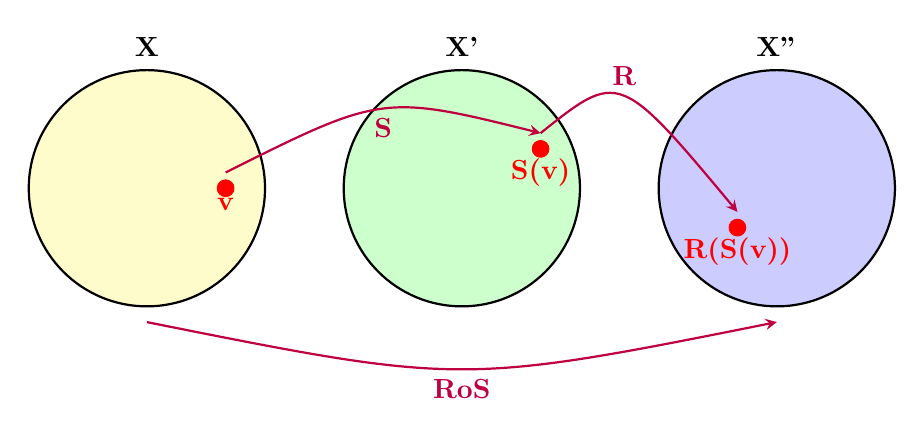
\begin{tikzpicture}

            % Draw sets A, B, C
            \draw[fill=yellow!20!white, draw=black, thick] (-4,0) ellipse (1.5cm);
            \draw[fill=green!20!white, draw=black, thick] (0,0) ellipse (1.5cm);
            \draw[fill=blue!20!white, draw=black, thick] (4,0) ellipse (1.5cm);
            
            % Labels for sets A, B, C
            \node at (-4,1.8) {\textbf{X}};
            \node at (0,1.8) {\textbf{X'}};
            \node at (4,1.8) {\textbf{X''}};
            
            % Elements inside sets
            \filldraw[red] (-3,0) circle (3pt) node[below] {\textbf{v}};
            \filldraw[red] (1,.5) circle (3pt) node[below] {\textbf{S(v)}};
            \filldraw[red] (3.5,-.5) circle (3pt) node[below] {\textbf{R(S(v))}};
            
            % Arrows for functions f, g, gof
            \draw[->, thick, purple] (-3,0.2) .. controls (-1,1.2) .. (1,.7) node[midway, below] {\textbf{S}};
            \draw[->, thick, purple] (1,.7) .. controls (2,1.5) .. (3.5,-.3) node[midway, above] {\textbf{R}};
            \draw[->, thick, purple] (-4,-1.7) .. controls (0,-2.5) .. (4,-1.7) node[midway, below] {\textbf{RoS}};
            
        \end{tikzpicture}

        In the above diagram, $X$ is the original data, $X'$ is the data after the stretching transformation, and $X''$ is the data after the rotation transformation. The arrows represent the transformations that progressively alter the data, and the final arrow represents the composition of the two transformations.

    \end{remark}

    Our goal is to find a systematic way of representing the composite transformation as a single matrix. From this example, let's track the transformations of the standard basis vectors.

    We start with the standard basis vectors $\vec{e}_1=\begin{bmatrix} 1 \\ 0 \end{bmatrix}$ and $\vec{e}_2=\begin{bmatrix} 0 \\ 1 \end{bmatrix}$, and apply the transformations in sequence.

    The stretching transformation matrix is $S=\begin{bmatrix} 1 & 0 \\ 0 & 2 \end{bmatrix}$, which tells us that the stretched basis vectors are $S\vec{e}_1=\begin{bmatrix}\answer{1} \\ 0 \end{bmatrix}$ and $S\vec{e}_2=\begin{bmatrix} 0 \\ \answer{2} \end{bmatrix}$.

    Whereas the rotation matrix $R=\begin{bmatrix} \cos 60 & -\sin 60 \\ \sin 60 & \cos 60 \end{bmatrix}$ would normally tell us where to map $\vec{e}_1$ and $\vec{e}_2$, to continue the tansformation we instead need to apply the matrix to $S\vec{e}_1$ and $S\vec{e}_2$.

    \begin{hint}\name{Notation}

        Don't let the notation fool you, $S\vec{e}_1$ and $S\vec{e}_2$ vectors, not matrices. Remember that multiplying a matrix by a vector gives you a transformed vector.

    \end{hint}

    \begin{question}

        What are the rotated vectors $RS\vec{e}_1$ and $RS\vec{e}_2$?

        \begin{solution}

            We have $S\vec{e}_1=\begin{bmatrix} 1 \\ 0 \end{bmatrix}$ and $S\vec{e}_2=\begin{bmatrix} 0 \\ 2 \end{bmatrix}$.

            Applying the rotation matrix $R$ to $S\vec{e}_1$ gives us $R(S\vec{e}_1)=\begin{bmatrix} \cos 60 & -\sin 60 \\ \sin 60 & \cos 60 \end{bmatrix}\begin{bmatrix} 1 \\ 0 \end{bmatrix}=\answer{1}\begin{bmatrix} \cos 60 \\ \sin 60 \end{bmatrix}+\answer{0}
            \begin{bmatrix} -\sin 60 \\ \cos 60 \end{bmatrix}=\begin{bmatrix} \cos 60 \\ \sin 60 \end{bmatrix}$.

            Applying the rotation matrix $R$ to $S\vec{e}_2$ gives us $R(S\vec{e}_2)=\begin{bmatrix} \cos 60 & -\sin 60 \\ \sin 60 & \cos 60 \end{bmatrix}\begin{bmatrix} 0 \\ 2 \end{bmatrix}=\answer{0}\begin{bmatrix} \cos 60 \\ \sin 60 \end{bmatrix}+\answer{2}
            \begin{bmatrix} -\sin 60 \\ \cos 60 \end{bmatrix}=\begin{bmatrix} -2\sin 60 \\ 2\cos 60 \end{bmatrix}$.

        \end{solution}

    \end{question}

    Putting this together, we see that the composite transformation matrix $RS$ is 
    
    $$RS=\begin{bmatrix} \cos 60 & -2\sin 60 \\ \sin 60 & 2\cos 60 \end{bmatrix}.$$

    Let's check that this matrix gives us the same result as the two transformations in sequence.

    Use the following MATLAB code to apply the composite transformation to the original smiley face.

    \begin{verbatim}

        load +linalg/face_points.mat

        RS = [cosd(60) -2*sind(60); sind(60) 2*cosd(60)];
        for i=1:length(face_points)
            face_points(i,:)=RS*face_points(i,:)';
        end
        linalg.plot_img_points(face_points)
    \end{verbatim}

    This yields the same smiley face as the two transformations in sequence!


    \end{example}

    \begin{remark}

        Note also that the notation we used to find the new basis vectors, $RS\vec{e}_1$ and $RS\vec{e}_2$ feels quite similar to notation used for scalar multiplication. For instance if $a=3$ and $b=4$ we would write $ab$ to mean $3\cdot 4$.

        This gives rise to the following definition of \emph{matrix multiplication}

        \begin{definition}

            Let $A$ be an $m\times n$ matrix and $B$ be an $n\times p$ matrix. The product $AB$ is an $m\times p$ matrix whose columns are given by 

            $$AB=\begin{bmatrix} A\vec{b}_1 & A\vec{b}_2 & \cdots & A\vec{b}_p \end{bmatrix}$$

            where $\vec{b}_1,\vec{b}_2,\ldots,\vec{b}_p$ are the columns of $B$.

        \end{definition}

        There is another, more standard definition of matrix multiplication that you'll often see in textbooks, which breaks down the operation for each entry rather than at each column. It's worth noting for efficiency, and that you'll see it in other contexts, however thinking about it as a column-wise operation is a good way to understand why matrix multiplication works the way it does.

        \begin{definition}\name{Entry-Wise Matrix Multiplication}

            Let $A$ be an $m\times n$ matrix and $B$ be an $n\times p$ matrix. The product $AB$ is an $m\times p$ matrix whose entries are given by 

            $$(AB)_{ij}=\sum_{k=1}^n A_{ik}B_{kj}.$$
        \end{definition}

    \end{remark}

    As usual, MATLAB has a built-in function for matrix multiplication, \texttt{A*B}, which will give you the same result as the column-wise definition of matrix multiplication. Let's check it on the previous example.

    \begin{example}

        Let's use MATLAB to check that the matrix $RS$ we found earlier is the same as the product of the matrices $R$ and $S$.

        \begin{verbatim}

            R = [cosd(60) -sind(60); sind(60) cosd(60)]
            S = [1 0; 0 2]
            RS = R*S
            RS
        \end{verbatim}

        This should yield the matrix $RS$ we found earlier, $\begin{bmatrix} \cos 60 & -2\sin 60 \\ \sin 60 & 2\cos 60 \end{bmatrix}$.
    \end{example}

    \begin{example}

        We're finally able to do all three of the transformations we initial set out to do: a vertical stretch by a factor of $2$, a $60^\circ$ rotation, and a reflection about the $y$-axis.

        Let's do it first in sequence, then as one transformation, and compare the results.

        \begin{enumerate}

            \item In Sequence: We already know the matrices for the stretch and rotation are $S=\begin{bmatrix} 1 & 0 \\ 0 & 2 \end{bmatrix}$ and $R=\begin{bmatrix} \cos 60 & -\sin 60 \\ \sin 60 & \cos 60 \end{bmatrix}$. The matrix for the reflection is $F=\begin{bmatrix} \answer{-1} & 0 \\ 0 & \answer{1} \end{bmatrix}$.
            
            Let's apply the transformations in sequence using MALTAB. 
            
            \begin{hint}\name{MATLAB}
            
            NOTE: The code will do it all in one for loop rather than three, but notice that each line within the for loop is applying each separate transformation to the smiley face points. 
            
            So first it will stretch the points, then the next line will rotate the already stretched points, then the next line will reflect the already stretched and rotated points.

            \end{hint}



            \texttt{load +linalg/face\textunderscore points.mat}

            \texttt{S = [1 0; 0 2]}

            \texttt{R = [cosd(60) -sind(60); sind(60) cosd(60)]}

            \texttt{F = [-1 0; 0 1]}

            \texttt{for i=1:length(face\textunderscore points)}

            \texttt{    face\textunderscore points(i,:)=}$\answer[format=string]{S}$\texttt{*face\textunderscore points(i,:)';}

            \texttt{        face\textunderscore points(i,:)=}$\answer[format=string]{R}$\texttt{*face\textunderscore points(i,:)';}

            \texttt{        face\textunderscore points(i,:)=}$\answer[format=string]{F}$\texttt{*face\textunderscore points(i,:)';}

            \texttt{end}

            \texttt{linalg.plot\textunderscore img\textunderscore points(face\textunderscore points)}

            \item Now we can do the same thing, but as one transformation. We'll call the composite matrix $M$.
            
            \vspace{1cm}
            
            \texttt{load +linalg/face\textunderscore points.mat}

            \texttt{R = [cosd(60) -sind(60); sind(60) cosd(60)]}

            \texttt{S = [1 0; 0 2]}

            \texttt{F = [-1 0; 0 1]}

            \texttt{M = }$\answer[format=string]{F}*\answer[format=string]{R}*\answer[format=string]{S}$

            \texttt{for i=1:length(face\textunderscore points)}

            $\qquad $\texttt{face\textunderscore points(i,:) = }$\answer[format=string]{M}$\texttt{*face\textunderscore points(i,:)';}

            \texttt{end}

            \texttt{linalg.plot\textunderscore img\textunderscore points(face\textunderscore points)}

        \end{enumerate}

        Hopefully both approaches got you the following:

        \begin{center}
            \includegraphics[width=\textwidth]{face_stretch_rotate_reflect.png}
        \end{center}

    \end{example}

\end{document}